\documentclass[a3paper,xelatex,english]{bxjsarticle}
\usepackage{pgfplots,pgfplotstable}
\pgfplotsset{ compat = newest }
\usepackage{tikz}
\usetikzlibrary{arrows.meta,bending,calc,shapes,positioning}
\usepackage{ascmac}
\usepackage{fancybox}
\usepackage{amsmath,amssymb}
\usepackage{algorithm}
\usepackage[edges]{forest}
\usepackage{array}
\usepackage{algpseudocode}
\usepackage{paralist}
\usepackage{cases}
\usepackage{fvextra}
\usepackage{colortbl}
\usepackage{xcolor}
\usepackage{fancyhdr}
\usepackage[explicit]{titlesec}
\usepackage{xspace}
\usepackage[many]{tcolorbox}
\usepackage{lastpage}
\usepackage{verbatim}
\usepackage{multirow}
\usepackage{censor}
\usepackage[unicode,pdftitle={Report of Entropy estimates based on NIST SP 800-90B non-IID track},setpagesize=false]{hyperref}
\usepackage[open,openlevel=4]{bookmark}
\newcommand\mib[1]{\boldsymbol{#1}}
\usepgfplotslibrary{patchplots}
%%%%%%%%%%%%%%%%%%%%%%%%%%%%%%%%%%%%%%%%%%%%%%%%%%%%%%%%%%%%%%%%%%%%%%%%%%%%%%%
%%%%%%
%%%%%% customize page numbering
%%%%%%
%%%%%%%%%%%%%%%%%%%%%%%%%%%%%%%%%%%%%%%%%%%%%%%%%%%%%%%%%%%%%%%%%%%%%%%%%%%%%%%
\fancypagestyle{mypagestylewithtotalpagenumbers}{
\lhead{}
\rhead{}
\cfoot{\thepage/\pageref{LastPage}}
\renewcommand{\headrulewidth}{0.0pt}
}
%%%%%%%%%%%%%%%%%%%%%%%%%%%%%%%%%%%%%%%%%%%%%%%%%%%%%%%%%%%%%%%%%%%%%%%%%%%%%%%
%%%%%%
%%%%%% output up to 4-th level
%%%%%%
%%%%%%%%%%%%%%%%%%%%%%%%%%%%%%%%%%%%%%%%%%%%%%%%%%%%%%%%%%%%%%%%%%%%%%%%%%%%%%%
\setcounter{secnumdepth}{4}
\setcounter{tocdepth}{4}
\setlength{\topmargin}{-1cm}
\setlength{\textheight}{37cm}
%%%%%%%%%%%%%%%%%%%%%%%%%%%%%%%%%%%%%%%%%%%%%%%%%%%%%%%%%%%%%%%%%%%%%%%%%%%%%%%
%%%%%%
%%%%%%
%%%%%%
%%%%%%%%%%%%%%%%%%%%%%%%%%%%%%%%%%%%%%%%%%%%%%%%%%%%%%%%%%%%%%%%%%%%%%%%%%%%%%%
%%%\renewcommand{ \figurename }{Figure }
%%%\renewcommand{ \tablename }{Table }
%%%\renewcommand{ \refname }{References}
%%%%%%%%%%%%%%%%%%%%%%%%%%%%%%%%%%%%%%%%%%%%%%%%%%%%%%%%%%%%%%%%%%%%%%%%%%%%%%%
%%%%%%
%%%%%%
%%%%%%
%%%%%%%%%%%%%%%%%%%%%%%%%%%%%%%%%%%%%%%%%%%%%%%%%%%%%%%%%%%%%%%%%%%%%%%%%%%%%%%
\definecolor{rowcolorlightblue}{RGB}{191,233,251}
\definecolor{bordercolordarkblue}{RGB}{0,163,243}
\definecolor{BleuDur}{RGB}{27,61,176}
\definecolor{Nigelle}{RGB}{0,133,201}
\definecolor{BleuFaience}{RGB}{105,171,219}
\definecolor{anotherlightblue}{RGB}{61,143,244}
%%%%%%%%%%%%%%%%%%%%%%%%%%%%%%%%%%%%%%%%%%%%%%%%%%%%%%%%%%%%%%%%%%%%%%%%%%%%%%%
%%%%%%
%%%%%%
%%%%%%
%%%%%%%%%%%%%%%%%%%%%%%%%%%%%%%%%%%%%%%%%%%%%%%%%%%%%%%%%%%%%%%%%%%%%%%%%%%%%%%
\def\chpcolor{BleuDur}
\def\chpcolortxt{BleuDur}
\def\sectionfont{\sffamily\LARGE}
%%%%%%%%%%%%%%%%%%%%%%%%%%%%%%%%%%%%%%%%%%%%%%%%%%%%%%%%%%%%%%%%%%%%%%%%%%%%%%%
%%%%%%
%%%%%%
%%%%%%
%%%%%%%%%%%%%%%%%%%%%%%%%%%%%%%%%%%%%%%%%%%%%%%%%%%%%%%%%%%%%%%%%%%%%%%%%%%%%%%
\makeatletter
%Section:
\def\@sectionstrut{\vrule\@width\z@\@height12.5\p@}
\def\@makesectionhead#1{%
  {\par\vspace{20pt}%
   \parindent 0pt\raggedleft\sectionfont
   \colorbox{\chpcolor}{%
     \parbox[t]{90pt}{\color{white}\@sectionstrut\@depth4.5\p@\hfill
       \ifnum\c@secnumdepth>\z@\thesection\fi}%
   }%
   \begin{minipage}[t]{\dimexpr\textwidth-90pt-2\fboxsep\relax}
   \color{\chpcolortxt}\@sectionstrut\hspace{5pt}#1
   \end{minipage}\par
   \vspace{10pt}%
  }
}
\def\section{\@afterindentfalse\secdef\@section\@ssection}
\def\@section[#1]#2{%
  \ifnum\c@secnumdepth>\m@ne
    \refstepcounter{section}%
    \addcontentsline{toc}{section}{\protect\numberline{\thesection}#1}%
  \else
    \phantomsection
    \addcontentsline{toc}{section}{#1}%
  \fi
  \sectionmark{#1}%
  \if@twocolumn
    \@topnewpage[\@makesectionhead{#2}]%
  \else
    \@makesectionhead{#2}\@afterheading
  \fi
}
\def\@ssection#1{%
  \if@twocolumn
    \@topnewpage[\@makesectionhead{#1}]%
  \else
    \@makesectionhead{#1}\@afterheading
  \fi
}
\makeatother
%%%%%%%%%%%%%%%%%%%%%%%%%%%%%%%%%%%%%%%%%%%%%%%%%%%%%%%%%%%%%%%%%%%%%%%%%%%%%%%
%%%%%%
%%%%%%
%%%%%%
%%%%%%%%%%%%%%%%%%%%%%%%%%%%%%%%%%%%%%%%%%%%%%%%%%%%%%%%%%%%%%%%%%%%%%%%%%%%%%%
\setlength{ \topmargin }{-1.5cm}
%%%%%%%%%%%%%%%%%%%%%%%%%%%%%%%%%%%%%%%%%%%%%%%%%%%%%%%%%%%%%%%%%%%%%%%%%%%%%%%
%%%%%%
%%%%%%
%%%%%%
%%%%%%%%%%%%%%%%%%%%%%%%%%%%%%%%%%%%%%%%%%%%%%%%%%%%%%%%%%%%%%%%%%%%%%%%%%%%%%%
\pagestyle{mypagestylewithtotalpagenumbers}
%%%%%%
%%%%%%
%%%%%%
\title{Report of Entropy estimates based on NIST SP 800-90B non-IID track}
\date{2023-Dec-17 11:06:32.099745}
\begin{document}
\StopCensoring
\maketitle
%%%%%%%%%%%%%%%%%%%%%%%%%%%%%%%%%%%%%%%%%%%%%%%%%%%%%%%%%%%%%%%%%%%%%%%%%%%%%%%
%%%%%%
%%%%%%%%%%%%%%%%%%%%%%%%%%%%%%%%%%%%%%%%%%%%%%%%%%%%%%%%%%%%%%%%%%%%%%%%%%%%%%%
\thispagestyle{mypagestylewithtotalpagenumbers}
%%%%%%%%%%%%%%%%%%%%%%%%%%%%%%%%%%%%%%%%%%%%%%%%%%%%%%%%%%%%%%%%%%%%%%%%%%%%%%%
%%%%%%
%%%%%%%%%%%%%%%%%%%%%%%%%%%%%%%%%%%%%%%%%%%%%%%%%%%%%%%%%%%%%%%%%%%%%%%%%%%%%%%
\section{Identification information}
\subsection{Identification of acquisition data from entropy source}
\renewcommand{\arraystretch}{1.8}
\begin{table}[h]
\caption{Identification information of acquisition data from entropy source}
\begin{center}
\begin{tabular}{|>{\columncolor{anotherlightblue}}p{2cm}|p{20.5cm}|}
\hline 
Path to the acquisition data & \verb|"D:\usr\SP800-90B_EntropyAssessment-master\bin\rand1_short.bin"| \\
\hline
SHA-256 hash value of the acquisition data [hex] & 
\begin{verbatim}
38144044 97a3b912 f8d3db6b c05a9933 8f0986cd 75fe54af 2a5f1bdb 0a12a583
\end{verbatim} 
\\
\hline
Last write time & 2021-Sep-20 10:22:44 \\
\hline
\end{tabular}
\end{center}
\end{table}
\renewcommand{\arraystretch}{1.8}
\begin{itemize}
		\item Name of the submitter of the acquisition data : 
		    \begin{Form}
		    \noindent
		    \TextField[name=NameOfSubmitter, multiline=false, bordercolor=bordercolordarkblue,width=12cm]{}
		    \end{Form}
		\item Brief explanation of the acquisition data (or entropy source) : \\
		    \begin{Form}
		    \noindent
		    \TextField[name=ExplanationOfAcquisitionData, multiline=true, bordercolor=bordercolordarkblue,width=\linewidth,height=1in]{}
		    \end{Form}
	\end{itemize} 
\subsection{Identification of analysis environment}
\renewcommand{\arraystretch}{1.8}
\begin{table}[h]
\caption{Identification information of analysis environment}
\begin{center}
\begin{tabular}{|>{\columncolor{anotherlightblue}}l|>{\columncolor{anotherlightblue}}l|p{12cm}|}
\hline 
Analysis tool & Name & Another entropy estimation tool with extensions \\
\cline{2-3}
\, & Versioning information & 1.0.52 \\
\cline{2-3}
\, & built as &  64-bit application \\
\cline{2-3}
\, & built by &  Intel C++ Compiler ( \verb|__INTEL_LLVM_COMPILER|: 20240000 ) \\
\cline{2-3}
\, & linked libraries &  Boost C++ 1.84.0 \\
\hline
Analysis environment & Hostname & \censor{PANTHERF340} \\
\cline{2-3}
\, & CPU information & Intel(R) Core(TM) i5-10500T CPU @ 2.30GHz \\
\cline{2-3}
\, &  Physical memory size & 65239 MiB \\
\cline{2-3}
\, &  OS information & Windows 10 or greater 64-bit \\
\cline{2-3}
\, &  Username & \censor{genya} \\
\hline
\end{tabular}
\end{center}
\end{table}
\renewcommand{\arraystretch}{1.4}
\subsection{Identification of analysis conditions}
\renewcommand{\arraystretch}{1.8}
\begin{table}[h]
\caption{Identification information of analysis conditions}
\begin{center}
\begin{tabular}{|>{\columncolor{anotherlightblue}}l|p{8cm}|}
\hline 
Number of samples & 10000 \\
\hline
Bits per sample & 1 \\
\hline
\end{tabular}
\end{center}
\end{table}
\renewcommand{\arraystretch}{1.4}
\subsection{Identification of analysis method}
NIST SP 800-90B \cite{SP80090B} 6.3 with corrections \cite{CorrectionsSP80090B} is applied
\clearpage
\section{Executive summary}
\subsection{Numerical results of min-entropy estimates based on non-IID track}
\pgfplotstableread{
section	y	y-min	y-max
6.3.1	0.961059	-0.000280871	       0
6.3.2	0.691464	0.00362392	0.695146
6.3.3	0.987596	0.000567574	0.987596
6.3.4	0.611716	       0	       0
6.3.5	0.867624	       0	       0
6.3.6	0.962626	       0	       0
6.3.7	0.952618	0.000280904	0.952899
6.3.8	0.943334	0.000277324	0.943611
6.3.9	0.961617	0.000280983	0.961898
6.3.10	0.961446	0.000281371	0.961728
}{\summarytableBinary}
\begin{table}[h]
\caption{Numerical results}
\begin{center}
\begin{tabular}{|l|c|c|}
\hline 
\rowcolor{anotherlightblue} %%
Estimator										& $H_{\textrm{bitstring}}$$^{\textrm{\,a}}$ & Notes to $H_{\textrm{bitstring}}$	\\ 
\cline{2-3}
\rowcolor{anotherlightblue} %%
\,												& [bit / 1 - bit] & \,		\\
\hline 
The Most Common Value Estimate					& 0.961059& see \ref{sec:Binary631} \\
\hline 
The Collision Estimate							& 0.691464& see \ref{sec:Binary632} \\
\hline 
The Markov Estimate								& 0.987596& see \ref{sec:Binary633} \\
\hline 
The Compression Estimate						& 0.611716& see \ref{sec:Binary634} \\
\hline 
The t-Tuple Estimate							& 0.867624& see \ref{sec:Binary635} \\
\hline 
The Longest Repeated Substring (LRS) Estimate	& 0.962626& see \ref{sec:Binary636} \\
\hline 
Multi Most Common in Window Prediction Estimate	& 0.952618& see \ref{sec:Binary637} \\
\hline 
The Lag Prediction Estimate						& 0.943334& see \ref{sec:Binary638} \\
\hline 
The MultiMMC Prediction Estimate				& 0.961617& see \ref{sec:Binary639} \\
\hline 
The LZ78Y Prediction Estimate					& 0.961446& see \ref{sec:Binary6310} \\
\hline \hline 
The intial entropy source estimate [bit / 1 -bit]	& \multicolumn{2}{|c|}{0.611716}	\\
$H_{I} = H_{\textrm{bitstring}}$ & \multicolumn{2}{|c|}{ \, } 	\\
\hline \hline 
\multicolumn{3}{|l|}{$^{\,a}$\quad Entropy estimate of the sequential dataset [source: NIST SP 800-90B \cite{SP80090B} 3.1.3]} \\
\hline 
\end{tabular}
\end{center}
\end{table}
\subsection{Visual comparison of min-entropy estimates from binary samples}
\begin{figure}[htbp]
\centering

\begin{tikzpicture} 
\begin{axis}
	[symbolic x coords={6.3.1,6.3.2,6.3.3,6.3.4,6.3.5,6.3.6,6.3.7,6.3.8,6.3.9,6.3.10},
	width=18cm,
	ymin=0,
	ymax=1,
	xlabel=Sub-sub-section of NIST SP 800-90B,
	ylabel={Estimated min-entropy $[$bit / 1-bit$]$},
	xtick=data]
\addplot+[forget plot,only marks] 
  plot[error bars/.cd, y dir=both, y explicit]
  table[x=section,y=y,y error plus expr=\thisrow{y-max},y error minus expr=\thisrow{y-min}] {\summarytableBinary};
\addplot+[Nigelle,no marks,sharp plot,update limits=false] 
coordinates {(6.3.1,0.611716) (6.3.10,0.611716)}
node[below] at (axis cs:6.3.5,0.611716) {Estimated min-entropy = 
0.611716};
\end{axis} 
\end{tikzpicture}

\caption{Estimated Min-Entropy using $\S$6.3 of NIST SP 800-90B}
\end{figure}
\clearpage
\section{Detailed results of analysis from original samples}
\subsection{The Most Common Value Estimate (NIST SP 800-90B Section 6.3.1)}\label{sec:Binary631}

\begin{figure}[htbp]
\centering

\begin{tikzpicture}
\begin{axis}[
	ybar,
	bar width=5pt,
	xmin=-0.125,
xmax=1.125,	ymin=0,
	width=20cm,
	xlabel=$x_i$,
	ylabel=\#$\{x_i \,\textrm{in} \,S\} / L$
]
\addplot coordinates {
(       0,   0.4992)
(       1,   0.5008)
};
\addplot+[Nigelle,no marks,sharp plot,update limits=false] 
coordinates {(0,0.5008) (1,0.5008)}
node[above] at (axis cs:0.5,0.5008) {\shortstack{$\hat{p}$ = 
0.5008\\($\rightarrow$ min-entropy = 0.961059 [bit / 1-bit])}};
\end{axis}
\end{tikzpicture}

\caption{Distribution of $x_i$}
\end{figure}
\subsubsection{Supplemental information for traceability}
\renewcommand{\arraystretch}{1.8}
\begin{table}[h]
\caption{Supplemental information for traceability (NIST SP 800-90B Section 6.3.1)}
\begin{center}
\begin{tabular}{|l|c|}
\hline 
\rowcolor{anotherlightblue} %%
Symbol				& Value \\ \hline 
mode				&     5008\\ \hline 
$\hat{p}$ 			&   0.5008\\ \hline
$p_u$				&  0.51368\\ \hline
\end{tabular}
\end{center}
\end{table}
\renewcommand{\arraystretch}{1.4}
\clearpage
\subsection{The Collision Estimate (NIST SP 800-90B Section 6.3.2)}\label{sec:Binary632}

\begin{figure}[htbp]
\centering

\begin{tikzpicture}
\begin{axis}[
	ybar,
	xmin=0,
	xtick={0, 1, 2, 3},
	ymin=0,
	width=20cm,
	xlabel=$t_{\nu}$,
	ylabel=occurrences of $t_{\nu}$
]
\addplot+[ybar] coordinates {
(       2,     2039)
(       3,     1974)
};
\addplot+[Nigelle,no marks,sharp plot,update limits=false] 
coordinates {(2.47157,2039) (2.47157,1)}
node[above right] at (axis cs:2.47157,2039) {$\bar{X}'$ = 2.47157};
\end{axis}
\end{tikzpicture}

\caption{Distribution of intermediate value $t_{\nu}$}
\end{figure}
\begin{figure}[htbp]
\centering

\begin{tikzpicture}[scale=12]
\draw[very thin,color=gray,dotted] (0,2) grid[step=0.25] (1,3);
\draw[->] (0, 2) -- (1.1,2) node[right] {$p$};
\draw[->] (0, 1.95) -- (0,3.05) node[above] {\shortstack{RHS of equation in step 7 \\$\equiv g(p)$}};
\draw[domain=0.5:1, smooth, variable=\x, color=blue] plot (\x,{2*(\x*(1-\x)+1)}) node[above right, xshift = 2mm, yshift = 2mm] {$g(p) = 2 \left[ p (1 - p) + 1 \right] $};
\draw[gray,loosely dotted] (  0.5,2.5) -- ( 0.0,2.5);
\draw[gray,loosely dotted] (  0.5,2.5) -- ( 0.5,2);
\draw (-0.1,  3) node {3} ;
\draw (-0.1,  2) node {2} ;
\draw (-0.1,  2.5) node {$\frac{5}{2}$} ;
\draw ( 0  ,  1.9) node {0} ;
\draw ( 0.5,  1.9) node {$\frac{1}{2}$} ;
\draw ( 1.0,  1.9) node {1} ;
%
%
\draw[Nigelle,dashed] ( 0, 2.47157) --(0.619225, 2.47157); 
\draw[Nigelle,dashed] ( 0.619225, 2) --(0.619225, 2.47157); 
\draw (0.619225, 2) node[below]{ \textcolor{Nigelle}{ \shortstack{ 0.619225 \\ 
($\rightarrow$ min-entropy = 0.691464 [bit / 1-bit]) 
} } }; 
\draw (0.125, 2.47157) node[below]{ \textcolor{Nigelle}{ $\bar{X}' = 2.47157$}  
}; 
%
%
\end{tikzpicture}
\caption{Solution to the equation in step 7}
\end{figure}
\clearpage
\subsubsection{Supplemental information for traceability}
\renewcommand{\arraystretch}{1.8}
\begin{table}[h]
\caption{Supplemental information for traceability (NIST SP 800-90B Section 6.3.2)}
\begin{center}
\begin{tabular}{|l|c|}
\hline 
\rowcolor{anotherlightblue} %%
Symbol				& Value \\ \hline 
$p$				& 0.619225\\ \hline 
$\bar{X}$ 		&   2.4919\\ \hline
$\bar{X}'$		&  2.47157\\ \hline
$\hat{\sigma}$		& 0.499997\\ \hline
\end{tabular}
\end{center}
\end{table}
\renewcommand{\arraystretch}{1.4}
\clearpage
\subsection{The Markov Estimate (NIST SP 800-90B Section 6.3.3)}\label{sec:Binary633}

\begin{figure}[htbp]
\begin{tikzpicture} 
\begin{axis}[
	xlabel=$i$,
	ylabel=$P_{i,j}$,
	width=10cm,
	xmin=-0.125,xmax=1.125,
	xtick={0, 1},
	legend style={at={(1,0.75)},anchor=north west},
	/pgf/number format/.cd,fixed,precision=6,
	scatter/classes={%
		a={mark=square*,blue},
		b={mark=square*,red},
		c={mark=square*,green},
		d={mark=square*,cyan}}]
	\addplot[scatter,only marks,%
		scatter src=explicit symbolic]%
	table[meta=label] {
x	y	label
 0	0.494891	a
 0	0.505109	b
 1	0.503594	c
 1	0.496406	d
	};
\legend{$P_{0,0}$, $P_{0,1}$, $P_{1,0}$, $P_{1,1}$}
\end{axis} 
\end{tikzpicture}
\caption{Transition probability $P_{i,j}$ of $\S$6.3.3 of NIST SP 800-90B}
\end{figure}
\begin{figure}[htbp]
\begin{tikzpicture} 
\begin{axis}[
	xlabel=Sequence index,
	ylabel=$-\log_{2}\left ( \textrm{Probability}\right ) / 128$,
	width=18cm,
	xmin=0.5,xmax=14.5,
	legend style={at={(1,1)},anchor=north west},
	/pgf/number format/.cd,fixed,precision=6,
	scatter/classes={%
		a={mark=square*,blue},
		b={mark=square*,red},
		c={mark=square*,green},
		d={mark=square*,cyan},
		e={mark=square*,magenta},
		f={mark=square*,yellow},
		g={mark=triangle*,blue},
		h={mark=triangle*,red},
		i={mark=triangle*,green},
		j={mark=triangle*,cyan},
		k={mark=triangle*,magenta},
		l={mark=triangle*,yellow},
		m={mark=o,blue},
		n={mark=o,red}}]
	\addplot[scatter,only marks,%
		scatter src=explicit symbolic]%
	table[meta=label] {
x	y	label
 1	 1.01472	a
	};
	\addplot[scatter,only marks,%
		scatter src=explicit symbolic]%
	table[meta=label] {
x	y	label
 2	0.987829	b
	};
	\addplot[scatter,only marks,%
		scatter src=explicit symbolic]%
	table[meta=label] {
x	y	label
 3	0.987794	c
	};
	\addplot[scatter,only marks,%
		scatter src=explicit symbolic]%
	table[meta=label] {
x	y	label
 4	 1.00999	d
	};
	\addplot[scatter,only marks,%
		scatter src=explicit symbolic]%
	table[meta=label] {
x	y	label
 5	 1.01449	e
	};
	\addplot[scatter,only marks,%
		scatter src=explicit symbolic]%
	table[meta=label] {
x	y	label
 6	0.987598	f
	};
	\addplot[scatter,only marks,%
		scatter src=explicit symbolic]%
	table[meta=label] {
x	y	label
 7	 1.01015	g
	};
	\addplot[scatter,only marks,%
		scatter src=explicit symbolic]%
	table[meta=label] {
x	y	label
 8	 1.01449	h
	};
	\addplot[scatter,only marks,%
		scatter src=explicit symbolic]%
	table[meta=label] {
x	y	label
 9	0.987596	i
	};
	\addplot[scatter,only marks,%
		scatter src=explicit symbolic]%
	table[meta=label] {
x	y	label
10	 1.01015	j
	};
	\addplot[scatter,only marks,%
		scatter src=explicit symbolic]%
	table[meta=label] {
x	y	label
11	 1.01426	k
	};
	\addplot[scatter,only marks,%
		scatter src=explicit symbolic]%
	table[meta=label] {
x	y	label
12	0.987793	l
	};
	\addplot[scatter,only marks,%
		scatter src=explicit symbolic]%
	table[meta=label] {
x	y	label
13	0.987758	m
	};
	\addplot[scatter,only marks,%
		scatter src=explicit symbolic]%
	table[meta=label] {
x	y	label
14	 1.01031	n
	};
\legend{$[$sequence index 1$]$ $0000 \cdots 0000$, $[$sequence index 2$]$ $0101 \cdots 0101001010 \cdots 1010$, $[$sequence index 3$]$ $0101 \cdots 0101101010 \cdots 1010$, $[$sequence index 4$]$ $0111 \cdots 1110$, $[$sequence index 5$]$ $0000 \cdots 0001$, $[$sequence index 6$]$ $0101 \cdots 0101$, $[$sequence index 7$]$ $0111 \cdots 1111$, $[$sequence index 8$]$ $1000 \cdots 0000$, $[$sequence index 9$]$ $1010 \cdots 1010$, $[$sequence index 10$]$ $1111 \cdots 1110$, $[$sequence index 11$]$ $1000 \cdots 0001$, $[$sequence index 12$]$ $1010 \cdots 1010100101 \cdots 0101$, $[$sequence index 13$]$ $1010 \cdots 1010110101 \cdots 0101$, $[$sequence index 14$]$ $1111 \cdots 1111$}
\end{axis} 
\end{tikzpicture}
\caption{Estimated Min-Entropy using $\S$6.3.3 of NIST SP 800-90B}
\end{figure}
\clearpage
\subsection{The Compression Estimate (NIST SP 800-90B Section 6.3.4)}\label{sec:Binary634}

\begin{figure}[htbp]
\centering

\begin{tikzpicture}
\begin{semilogxaxis}[
	width=20cm,
	xlabel=$D_{i}$,
	ylabel=number of $D_{i}$,
	log basis x={2}
]
\addplot coordinates {
(       1,        9)
(       2,       17)
(       3,       11)
(       4,        7)
(       5,       10)
(       6,        9)
(       7,        7)
(       8,        7)
(       9,       11)
(      10,        2)
(      11,       10)
(      12,       10)
(      13,        6)
(      14,       10)
(      15,        7)
(      16,        7)
(      17,        6)
(      18,       12)
(      19,        9)
(      20,        2)
(      21,        7)
(      22,        8)
(      23,        4)
(      24,       10)
(      25,       14)
(      26,       12)
(      27,        6)
(      28,        3)
(      29,        8)
(      30,        7)
(      31,        9)
(      32,        7)
(      33,        6)
(      34,        7)
(      35,        7)
(      36,        4)
(      37,        4)
(      38,        3)
(      39,       12)
(      40,        5)
(      41,        5)
(      42,        5)
(      43,        7)
(      44,        5)
(      45,        4)
(      46,        4)
(      47,        1)
(      48,        6)
(      49,        8)
(      50,        6)
(      51,        3)
(      52,        3)
(      53,        1)
(      54,        3)
(      55,        7)
(      57,        7)
(      58,        4)
(      59,        7)
(      60,        3)
(      61,        3)
(      62,        5)
(      63,        6)
(      64,        7)
(      65,        1)
(      66,        3)
(      67,        3)
(      68,        2)
(      69,        7)
(      70,        5)
(      71,        2)
(      72,        5)
(      73,        5)
(      75,        5)
(      76,        1)
(      77,        3)
(      78,        6)
(      80,        3)
(      81,        1)
(      82,        6)
(      83,        2)
(      84,        2)
(      85,        2)
(      86,        2)
(      87,        6)
(      88,        2)
(      89,        3)
(      90,        5)
(      91,        2)
(      92,        3)
(      94,        5)
(      96,        2)
(      97,        3)
(      98,        1)
(      99,        2)
(     101,        1)
(     102,        5)
(     103,        3)
(     104,        2)
(     105,        2)
(     106,        3)
(     107,        1)
(     108,        2)
(     109,        4)
(     110,        3)
(     112,        1)
(     113,        2)
(     114,        6)
(     115,        2)
(     116,        1)
(     117,        1)
(     119,        3)
(     120,        3)
(     121,        1)
(     122,        1)
(     123,        1)
(     125,        1)
(     126,        4)
(     128,        2)
(     129,        2)
(     130,        2)
(     131,        2)
(     133,        2)
(     136,        2)
(     137,        1)
(     138,        1)
(     139,        1)
(     140,        3)
(     142,        1)
(     143,        1)
(     144,        1)
(     145,        1)
(     146,        2)
(     148,        2)
(     150,        1)
(     151,        1)
(     152,        1)
(     153,        1)
(     155,        1)
(     160,        1)
(     162,        1)
(     164,        1)
(     167,        4)
(     168,        1)
(     170,        1)
(     172,        2)
(     174,        1)
(     175,        1)
(     176,        3)
(     177,        1)
(     178,        1)
(     185,        1)
(     187,        2)
(     188,        1)
(     191,        2)
(     193,        2)
(     196,        2)
(     197,        1)
(     198,        2)
(     201,        3)
(     206,        1)
(     209,        1)
(     210,        3)
(     213,        2)
(     217,        1)
(     218,        1)
(     227,        1)
(     228,        2)
(     248,        1)
(     260,        1)
(     263,        1)
(     268,        1)
(     278,        2)
(     283,        1)
(     287,        1)
(     290,        1)
(     292,        1)
(     296,        1)
(     306,        1)
(     327,        1)
(     427,        1)
};
\addplot+[Nigelle,no marks,sharp plot,update limits=false] 
coordinates {(5.23228,17) (5.23228,1)}
node[above right] at (axis cs:5.23228,17) {\shortstack{$\bar{X}$ = 5.23228, \,$\hat{\sigma}=$1.02952\\($\rightarrow$ min-entropy = 0.611716 [bit / 1-bit])}};
\end{semilogxaxis}
\end{tikzpicture}

\caption{Distribution of intermediate value $D_{i}$}
\end{figure}
\subsubsection{Supplemental information for traceability}
\renewcommand{\arraystretch}{1.8}
\begin{table}[h]
\caption{Supplemental information for traceability (NIST SP 800-90B Section 6.3.4)}
\begin{center}
\begin{tabular}{|l|c|}
\hline 
\rowcolor{anotherlightblue} %%
Symbol				& Value \\ \hline 
$p$				& 0.0785472\\ \hline 
$\bar{X}$ 		&  5.23228\\ \hline
$\hat{\sigma}$		&  1.02952\\ \hline
$\bar{X}'$ 		&  5.12953\\ \hline
\end{tabular}
\end{center}
\end{table}
\renewcommand{\arraystretch}{1.4}
\clearpage
\subsection{The t-tuple Estimate (NIST SP 800-90B Section 6.3.5)}\label{sec:Binary635}

\begin{figure}[htbp]
\centering

\begin{tikzpicture}
\begin{semilogyaxis}[
	width=20cm,
	xlabel=$i$,
	ylabel=$Q \lbrack i \rbrack $
]
\addplot coordinates {
(   1, 5008)
(   2, 2522)
(   3, 1294)
(   4, 686)
(   5, 367)
(   6, 197)
(   7, 106)
(   8, 63)
(   9, 36)
};
\end{semilogyaxis}
\end{tikzpicture}

\caption{Intermediate value $Q[i]$ \, in $\S$6.3.5 of NIST SP 800-90B}
\end{figure}
\begin{figure}[htbp]
\centering

\begin{tikzpicture}
\begin{axis}[
	width=20cm,
	xlabel=$i$,
	ylabel=$\left( P \lbrack i \rbrack \right)^{1/i}$,
	/pgf/number format/.cd,fixed,precision=6
]
\addplot coordinates {
(   1,   0.5008)
(   2,  0.50222)
(   3, 0.505833)
(   4, 0.511816)
(   5, 0.516378)
(   6, 0.519733)
(   7, 0.522322)
(   8,  0.53083)
(   9, 0.535201)
};
\addplot+[Nigelle,no marks,sharp plot,update limits=false] 
coordinates {(1,0.535201) (9,0.535201)}
node[above left] at (axis cs:9,0.535201) {\shortstack{$\hat{p}_{\textrm{max}}$ = 0.535201\\($\rightarrow$ min-entropy = 0.867624 [bit / 1-bit])}};
\end{axis}
\end{tikzpicture}

\caption{$P[i]^{1/i}$ \, in $\S$6.3.5 of NIST SP 800-90B}
\end{figure}
\clearpage
\subsubsection{Supplemental information for traceability}
\renewcommand{\arraystretch}{1.8}
\begin{table}[h]
\caption{Supplemental information for traceability (NIST SP 800-90B Section 6.3.5)}
\begin{center}
\begin{tabular}{|l|c|}
\hline 
\rowcolor{anotherlightblue} %%
Symbol				& Value \\ \hline 
$t$				&        9\\ \hline 
$\hat{p}_{\textrm{max}}$ 			& 0.535201\\ \hline
$p_u$				& 0.548049\\ \hline
\end{tabular}
\end{center}
\end{table}
\renewcommand{\arraystretch}{1.4}
\clearpage
\subsection{The LRS Estimate (NIST SP 800-90B Section 6.3.6)}\label{sec:Binary636}

\begin{figure}[htbp]
\centering

\begin{tikzpicture}
\begin{axis}[
	view/h=160,
	colormap/bluered, colorbar horizontal,
	width=20cm,
	ymin=2,
	xlabel=$W$,
	ylabel=$C_i$,
	zlabel=multiplicity,
]
\addplot3[surf, mesh/ordering=y varies, shader=faceted interp] coordinates {
(  10,   2,       2)  (  10,   3,      10)  (  10,   4,      18)  (  10,   5,      43)  (  10,   6,      82)  (  10,   7,      89)  (  10,   8,     129)  (  10,   9,     124)  (  10,  10,     130)  (  10,  11,     124)  (  10,  12,      83)  (  10,  13,      70)  (  10,  14,      46)  (  10,  15,      28)  (  10,  16,      24)  (  10,  17,      11)  (  10,  18,       5)  (  10,  19,       0)  (  10,  20,       2)  (  10,  21,       1)  (  10,  22,       1)  (  10,  23,       0)  (  10,  24,       0)  (  10,  25,       0)  (  10,  26,       0)  (  10,  27,       0)  (  10,  28,       1)  

(  11,   2,     174)  (  11,   3,     306)  (  11,   4,     385)  (  11,   5,     334)  (  11,   6,     296)  (  11,   7,     211)  (  11,   8,     124)  (  11,   9,      61)  (  11,  10,      33)  (  11,  11,      17)  (  11,  12,       6)  (  11,  13,       0)  (  11,  14,       0)  (  11,  15,       1)  (  11,  16,       1)  (  11,  17,       1)  (  11,  18,       0)  (  11,  19,       0)  (  11,  20,       0)  (  11,  21,       0)  (  11,  22,       0)  (  11,  23,       0)  (  11,  24,       0)  (  11,  25,       0)  (  11,  26,       0)  (  11,  27,       0)  (  11,  28,       0)  

(  12,   2,    1093)  (  12,   3,     893)  (  12,   4,     485)  (  12,   5,     258)  (  12,   6,     113)  (  12,   7,      31)  (  12,   8,      12)  (  12,   9,       6)  (  12,  10,       2)  (  12,  11,       0)  (  12,  12,       0)  (  12,  13,       0)  (  12,  14,       0)  (  12,  15,       0)  (  12,  16,       0)  (  12,  17,       0)  (  12,  18,       0)  (  12,  19,       0)  (  12,  20,       0)  (  12,  21,       0)  (  12,  22,       0)  (  12,  23,       0)  (  12,  24,       0)  (  12,  25,       0)  (  12,  26,       0)  (  12,  27,       0)  (  12,  28,       0)  

(  13,   2,    1776)  (  13,   3,     714)  (  13,   4,     236)  (  13,   5,      55)  (  13,   6,      11)  (  13,   7,       2)  (  13,   8,       0)  (  13,   9,       0)  (  13,  10,       0)  (  13,  11,       0)  (  13,  12,       0)  (  13,  13,       0)  (  13,  14,       0)  (  13,  15,       0)  (  13,  16,       0)  (  13,  17,       0)  (  13,  18,       0)  (  13,  19,       0)  (  13,  20,       0)  (  13,  21,       0)  (  13,  22,       0)  (  13,  23,       0)  (  13,  24,       0)  (  13,  25,       0)  (  13,  26,       0)  (  13,  27,       0)  (  13,  28,       0)  

(  14,   2,    1619)  (  14,   3,     337)  (  14,   4,      51)  (  14,   5,       8)  (  14,   6,       0)  (  14,   7,       0)  (  14,   8,       0)  (  14,   9,       0)  (  14,  10,       0)  (  14,  11,       0)  (  14,  12,       0)  (  14,  13,       0)  (  14,  14,       0)  (  14,  15,       0)  (  14,  16,       0)  (  14,  17,       0)  (  14,  18,       0)  (  14,  19,       0)  (  14,  20,       0)  (  14,  21,       0)  (  14,  22,       0)  (  14,  23,       0)  (  14,  24,       0)  (  14,  25,       0)  (  14,  26,       0)  (  14,  27,       0)  (  14,  28,       0)  

(  15,   2,    1091)  (  15,   3,     109)  (  15,   4,      10)  (  15,   5,       0)  (  15,   6,       0)  (  15,   7,       0)  (  15,   8,       0)  (  15,   9,       0)  (  15,  10,       0)  (  15,  11,       0)  (  15,  12,       0)  (  15,  13,       0)  (  15,  14,       0)  (  15,  15,       0)  (  15,  16,       0)  (  15,  17,       0)  (  15,  18,       0)  (  15,  19,       0)  (  15,  20,       0)  (  15,  21,       0)  (  15,  22,       0)  (  15,  23,       0)  (  15,  24,       0)  (  15,  25,       0)  (  15,  26,       0)  (  15,  27,       0)  (  15,  28,       0)  

(  16,   2,     621)  (  16,   3,      41)  (  16,   4,       0)  (  16,   5,       0)  (  16,   6,       0)  (  16,   7,       0)  (  16,   8,       0)  (  16,   9,       0)  (  16,  10,       0)  (  16,  11,       0)  (  16,  12,       0)  (  16,  13,       0)  (  16,  14,       0)  (  16,  15,       0)  (  16,  16,       0)  (  16,  17,       0)  (  16,  18,       0)  (  16,  19,       0)  (  16,  20,       0)  (  16,  21,       0)  (  16,  22,       0)  (  16,  23,       0)  (  16,  24,       0)  (  16,  25,       0)  (  16,  26,       0)  (  16,  27,       0)  (  16,  28,       0)  

(  17,   2,     335)  (  17,   3,      10)  (  17,   4,       0)  (  17,   5,       0)  (  17,   6,       0)  (  17,   7,       0)  (  17,   8,       0)  (  17,   9,       0)  (  17,  10,       0)  (  17,  11,       0)  (  17,  12,       0)  (  17,  13,       0)  (  17,  14,       0)  (  17,  15,       0)  (  17,  16,       0)  (  17,  17,       0)  (  17,  18,       0)  (  17,  19,       0)  (  17,  20,       0)  (  17,  21,       0)  (  17,  22,       0)  (  17,  23,       0)  (  17,  24,       0)  (  17,  25,       0)  (  17,  26,       0)  (  17,  27,       0)  (  17,  28,       0)  

(  18,   2,     174)  (  18,   3,       0)  (  18,   4,       0)  (  18,   5,       0)  (  18,   6,       0)  (  18,   7,       0)  (  18,   8,       0)  (  18,   9,       0)  (  18,  10,       0)  (  18,  11,       0)  (  18,  12,       0)  (  18,  13,       0)  (  18,  14,       0)  (  18,  15,       0)  (  18,  16,       0)  (  18,  17,       0)  (  18,  18,       0)  (  18,  19,       0)  (  18,  20,       0)  (  18,  21,       0)  (  18,  22,       0)  (  18,  23,       0)  (  18,  24,       0)  (  18,  25,       0)  (  18,  26,       0)  (  18,  27,       0)  (  18,  28,       0)  

(  19,   2,      92)  (  19,   3,       0)  (  19,   4,       0)  (  19,   5,       0)  (  19,   6,       0)  (  19,   7,       0)  (  19,   8,       0)  (  19,   9,       0)  (  19,  10,       0)  (  19,  11,       0)  (  19,  12,       0)  (  19,  13,       0)  (  19,  14,       0)  (  19,  15,       0)  (  19,  16,       0)  (  19,  17,       0)  (  19,  18,       0)  (  19,  19,       0)  (  19,  20,       0)  (  19,  21,       0)  (  19,  22,       0)  (  19,  23,       0)  (  19,  24,       0)  (  19,  25,       0)  (  19,  26,       0)  (  19,  27,       0)  (  19,  28,       0)  

(  20,   2,      47)  (  20,   3,       0)  (  20,   4,       0)  (  20,   5,       0)  (  20,   6,       0)  (  20,   7,       0)  (  20,   8,       0)  (  20,   9,       0)  (  20,  10,       0)  (  20,  11,       0)  (  20,  12,       0)  (  20,  13,       0)  (  20,  14,       0)  (  20,  15,       0)  (  20,  16,       0)  (  20,  17,       0)  (  20,  18,       0)  (  20,  19,       0)  (  20,  20,       0)  (  20,  21,       0)  (  20,  22,       0)  (  20,  23,       0)  (  20,  24,       0)  (  20,  25,       0)  (  20,  26,       0)  (  20,  27,       0)  (  20,  28,       0)  

(  21,   2,      20)  (  21,   3,       0)  (  21,   4,       0)  (  21,   5,       0)  (  21,   6,       0)  (  21,   7,       0)  (  21,   8,       0)  (  21,   9,       0)  (  21,  10,       0)  (  21,  11,       0)  (  21,  12,       0)  (  21,  13,       0)  (  21,  14,       0)  (  21,  15,       0)  (  21,  16,       0)  (  21,  17,       0)  (  21,  18,       0)  (  21,  19,       0)  (  21,  20,       0)  (  21,  21,       0)  (  21,  22,       0)  (  21,  23,       0)  (  21,  24,       0)  (  21,  25,       0)  (  21,  26,       0)  (  21,  27,       0)  (  21,  28,       0)  

(  22,   2,       8)  (  22,   3,       0)  (  22,   4,       0)  (  22,   5,       0)  (  22,   6,       0)  (  22,   7,       0)  (  22,   8,       0)  (  22,   9,       0)  (  22,  10,       0)  (  22,  11,       0)  (  22,  12,       0)  (  22,  13,       0)  (  22,  14,       0)  (  22,  15,       0)  (  22,  16,       0)  (  22,  17,       0)  (  22,  18,       0)  (  22,  19,       0)  (  22,  20,       0)  (  22,  21,       0)  (  22,  22,       0)  (  22,  23,       0)  (  22,  24,       0)  (  22,  25,       0)  (  22,  26,       0)  (  22,  27,       0)  (  22,  28,       0)  

(  23,   2,       3)  (  23,   3,       0)  (  23,   4,       0)  (  23,   5,       0)  (  23,   6,       0)  (  23,   7,       0)  (  23,   8,       0)  (  23,   9,       0)  (  23,  10,       0)  (  23,  11,       0)  (  23,  12,       0)  (  23,  13,       0)  (  23,  14,       0)  (  23,  15,       0)  (  23,  16,       0)  (  23,  17,       0)  (  23,  18,       0)  (  23,  19,       0)  (  23,  20,       0)  (  23,  21,       0)  (  23,  22,       0)  (  23,  23,       0)  (  23,  24,       0)  (  23,  25,       0)  (  23,  26,       0)  (  23,  27,       0)  (  23,  28,       0)  

(  24,   2,       2)  (  24,   3,       0)  (  24,   4,       0)  (  24,   5,       0)  (  24,   6,       0)  (  24,   7,       0)  (  24,   8,       0)  (  24,   9,       0)  (  24,  10,       0)  (  24,  11,       0)  (  24,  12,       0)  (  24,  13,       0)  (  24,  14,       0)  (  24,  15,       0)  (  24,  16,       0)  (  24,  17,       0)  (  24,  18,       0)  (  24,  19,       0)  (  24,  20,       0)  (  24,  21,       0)  (  24,  22,       0)  (  24,  23,       0)  (  24,  24,       0)  (  24,  25,       0)  (  24,  26,       0)  (  24,  27,       0)  (  24,  28,       0)  

(  25,   2,       1)  (  25,   3,       0)  (  25,   4,       0)  (  25,   5,       0)  (  25,   6,       0)  (  25,   7,       0)  (  25,   8,       0)  (  25,   9,       0)  (  25,  10,       0)  (  25,  11,       0)  (  25,  12,       0)  (  25,  13,       0)  (  25,  14,       0)  (  25,  15,       0)  (  25,  16,       0)  (  25,  17,       0)  (  25,  18,       0)  (  25,  19,       0)  (  25,  20,       0)  (  25,  21,       0)  (  25,  22,       0)  (  25,  23,       0)  (  25,  24,       0)  (  25,  25,       0)  (  25,  26,       0)  (  25,  27,       0)  (  25,  28,       0)  

};
\end{axis}
\end{tikzpicture}

\caption{Estimated $W$-tuple collision probability in Step 3 of $\S6.3.6$ of NIST SP 800-90B}
\end{figure}
\begin{figure}[htbp]
\centering

\begin{tikzpicture}
\begin{axis}[
	width=20cm,
	xlabel=$W$,
	ylabel=$\left( P_W \right) ^{i/W}$,
    ticklabel style={
        % change "directory" to the number format
        /pgf/number format/.cd,
            fixed,
        % change "directory" back to tikz
        /tikz/.cd,
    },
	yticklabel style = { /pgf/number format/precision=6 }
]
\addplot  coordinates {
(  10, 0.500086)
(  11, 0.500177)
(  12, 0.500242)
(  13, 0.500017)
(  14, 0.499676)
(  15, 0.499035)
(  16, 0.499312)
(  17, 0.498801)
(  18, 0.497553)
(  19, 0.499152)
(  20, 0.499737)
(  21, 0.495931)
(  22, 0.491113)
(  23, 0.485391)
(  24, 0.491856)
(  25, 0.492183)
};
\addplot+[Nigelle,no marks,sharp plot,update limits=false] 
coordinates {(10,0.500242) (25,0.500242)}
node[above, xshift=10mm] at (axis cs:12,0.500242) {\shortstack{$\hat{p}$ = 0.500242 \\($\rightarrow$ min-entropy = 0.962626 [bit / 1-bit])}};
\end{axis}
\end{tikzpicture}

\caption{Estimated average collision probability per string symbol in Step 3 of $\S6.3.6$ of NIST SP 800-90B}
\end{figure}
\clearpage
\subsubsection{Supplemental information for traceability}
\renewcommand{\arraystretch}{1.8}
\begin{table}[h]
\caption{Supplemental information for traceability (NIST SP 800-90B Section 6.3.6)}
\begin{center}
\begin{tabular}{|l|c|}
\hline 
\rowcolor{anotherlightblue} %%
Symbol				& Value \\ \hline 
$u$				&       10\\ \hline 
$v$				&       25\\ \hline 
$\hat{p}$ 			& 0.500242\\ \hline
$p_u$				& 0.513122\\ \hline
\end{tabular}
\end{center}
\end{table}
\renewcommand{\arraystretch}{1.4}
\clearpage
\subsection{Multi Most Common in Window Prediction Estimate (NIST SP 800-90B Section 6.3.7)}\label{sec:Binary637}

\begin{figure}[htbp]
\centering

\begin{tikzpicture}
\begin{axis}[
	ybar,
	xmin=0,
	ymin=0,
	width=20cm,
	xlabel=length of run of ones in $correct$,
	ylabel=occurrences
]
\addplot+[ybar] coordinates {
(       1,       1)
(       2,       1)
(       4,       1)
(       5,       1)
(       8,       1)
(       9,       1)
(      10,       1)
(      12,       1)
};
\addplot+[Nigelle,no marks,sharp plot,update limits=false] 
coordinates {(12, 1) (12, 1)}
node[above left] at (axis cs:12, 1) {\shortstack{$r - 1$ = 12 
\\($\rightarrow$ min-entropy = 0.952618 [bit / 1-bit])}};
\end{axis}
\end{tikzpicture}
\caption{Distribution of $correct$}
\end{figure}
\subsubsection{Supplemental information for traceability}
\renewcommand{\arraystretch}{1.8}
\begin{table}[h]
\caption{Supplemental information for traceability (NIST SP 800-90B Section 6.3.7)}
\begin{center}
\begin{tabular}{|l|c|}
\hline 
\rowcolor{anotherlightblue} %%
Symbol				& Value \\ \hline 
$N$				& 9937\\ \hline 
$C$				& 5006\\ \hline 
$P_{\textrm{global}}$				& 0.503774\\ \hline 
$P'_{\textrm{global}}$			& 0.516694\\ \hline 
$r$				& 13\\ \hline 
$P_{\textrm{local}}$ 			& 0.357828\\ \hline
\end{tabular}
\end{center}
\end{table}
\renewcommand{\arraystretch}{1.4}
\clearpage
\subsection{Lag Prediction Estimate (NIST SP 800-90B Section 6.3.8)}\label{sec:Binary638}

\begin{figure}[htbp]
\centering

\begin{tikzpicture}
\begin{axis}[
	ybar,
	xmin=0,
	ymin=0,
	width=20cm,
	xlabel=length of run of ones in $correct$,
	ylabel=occurrences
]
\addplot+[ybar] coordinates {
(       1,       1)
(       2,       1)
(       3,       1)
(       6,       1)
(       9,       1)
(      17,       1)
};
\addplot+[Nigelle,no marks,sharp plot,update limits=false] 
coordinates {(17, 1) (17, 1)}
node[above left] at (axis cs:17, 1) {\shortstack{$r - 1$ = 17 
\\($\rightarrow$ min-entropy = 0.943334 [bit / 1-bit])}};
\end{axis}
\end{tikzpicture}
\caption{Distribution of $correct$}
\end{figure}
\subsubsection{Supplemental information for traceability}
\renewcommand{\arraystretch}{1.8}
\begin{table}[h]
\caption{Supplemental information for traceability (NIST SP 800-90B Section 6.3.8)}
\begin{center}
\begin{tabular}{|l|c|}
\hline 
\rowcolor{anotherlightblue} %%
Symbol				& Value \\ \hline 
$N$				& 9999\\ \hline 
$C$				& 5071\\ \hline 
$P_{\textrm{global}}$				& 0.507151\\ \hline 
$P'_{\textrm{global}}$			&  0.52003\\ \hline 
$r$				& 18\\ \hline 
$P_{\textrm{local}}$ 			& 0.481593\\ \hline
\end{tabular}
\end{center}
\end{table}
\renewcommand{\arraystretch}{1.4}
\clearpage
\subsection{The MultiMMC Prediction Estimate (NIST SP 800-90B Section 6.3.9)}\label{sec:Binary639}

\begin{figure}[htbp]
\centering

\begin{tikzpicture}
\begin{axis}[
	ybar,
	xmin=0,
	ymin=0,
	width=20cm,
	xlabel=length of run of ones in $correct$,
	ylabel=occurrences
]
\addplot+[ybar] coordinates {
(       1,       1)
(       2,       1)
(       3,       2)
(       4,       1)
(       5,       1)
(       7,       1)
(       8,       1)
(       9,       1)
(      18,       1)
};
\addplot+[Nigelle,no marks,sharp plot,update limits=false] 
coordinates {(18, 1) (18, 1) }
node[above left] at (axis cs:18, 1) {\shortstack{$r - 1$ = 18 
\\($\rightarrow$ min-entropy = 0.961617 [bit / 1-bit])}};
\end{axis}
\end{tikzpicture}
\caption{Distribution of $correct$}
\end{figure}
\subsubsection{Supplemental information for traceability}
\renewcommand{\arraystretch}{1.8}
\begin{table}[h]
\caption{Supplemental information for traceability (NIST SP 800-90B Section 6.3.9)}
\begin{center}
\begin{tabular}{|l|c|}
\hline 
\rowcolor{anotherlightblue} %%
Symbol				& Value \\ \hline 
$N$				& 9998\\ \hline 
$C$				& 5005\\ \hline 
$P_{\textrm{global}}$				&   0.5006\\ \hline 
$P'_{\textrm{global}}$			& 0.513481\\ \hline 
$r$				& 19\\ \hline 
$P_{\textrm{local}}$ 			& 0.501512\\ \hline
\end{tabular}
\end{center}
\end{table}
\renewcommand{\arraystretch}{1.4}
\clearpage
\subsection{The LZ78Y Prediction Estimate (NIST SP 800-90B Section 6.3.10)}\label{sec:Binary6310}

\begin{figure}[htbp]
\centering

\begin{tikzpicture}
\begin{axis}[
	ybar,
	xmin=0,
	ymin=0,
	width=20cm,
	xlabel=length of run of ones in $correct$,
	ylabel=occurrences
]
\addplot+[ybar] coordinates {
(       4,       1)
(       5,       1)
(       7,       1)
(       8,       1)
(       9,       1)
(      18,       1)
};
\addplot+[Nigelle,no marks,sharp plot,update limits=false] 
coordinates {(18, 1) (18, 1)}
node[above left] at (axis cs:18, 1){\shortstack{$r - 1$ = 18 
\\($\rightarrow$ min-entropy = 0.961446 [bit / 1-bit])}};
\end{axis}
\end{tikzpicture}
\caption{Distribution of $correct$}
\end{figure}
\subsubsection{Supplemental information for traceability}
\renewcommand{\arraystretch}{1.8}
\begin{table}[h]
\caption{Supplemental information for traceability (NIST SP 800-90B Section 6.3.10)}
\begin{center}
\begin{tabular}{|l|c|}
\hline 
\rowcolor{anotherlightblue} %%
Symbol				& Value \\ \hline 
$N$				& 9983\\ \hline 
$C$				& 4998\\ \hline 
$P_{\textrm{global}}$				& 0.500651\\ \hline 
$P'_{\textrm{global}}$			& 0.513542\\ \hline 
$r$				& 19\\ \hline 
$P_{\textrm{local}}$ 			& 0.501554\\ \hline
\end{tabular}
\end{center}
\end{table}
\renewcommand{\arraystretch}{1.4}
\begin{thebibliography}{99}
% 1
\bibitem{SP80090B}
Meltem S\"{o}nmez Turan,
Elaine Barker,
John Kelsey,
Kerry A. McKay,
Mary L. Baish,
Mike Boyle
\textit{Recommendation for the Entropy Sources Used for Random Bit Generation},
NIST Special Publication 800-90B, Jan. 2018 
\url{https://nvlpubs.nist.gov/nistpubs/SpecialPublications/NIST.SP.800-90B.pdf}
% 2
\bibitem{CorrectionsSP80090B}
G. Sakurai, \textit{Proposed list of corrections for NIST SP 800-90B 6.3 Estimators}, Dec. 2022 
\url{https://github.com/g-g-sakura/AnotherEntropyEstimationTool/blob/main/documentation/ProposedListOfCorrections_SP800-90B.pdf}
\end{thebibliography}
\end{document}
